\documentclass[11pt,a4paper]{article}

\usepackage[utf8]{inputenc}
\usepackage[T1]{fontenc}
\usepackage[spanish]{babel}
\usepackage{graphicx}
\usepackage[margin=2.2cm]{geometry}
\usepackage{amsmath}

\begin{document}

\title{Correlaci\'on angular $\gamma$-$\gamma$ del $^{60}$Co}
\author{An\'alisis experimental}
\date{\today}
\maketitle

\section{Espectros individuales}

La Figura~\ref{fig:individuales} muestra los espectros completos de
coincidencia para cada \'angulo medido, con las posiciones de los picos
de 1173~keV y 1332~keV indicadas.

\begin{figure}[ht]
  \centering
  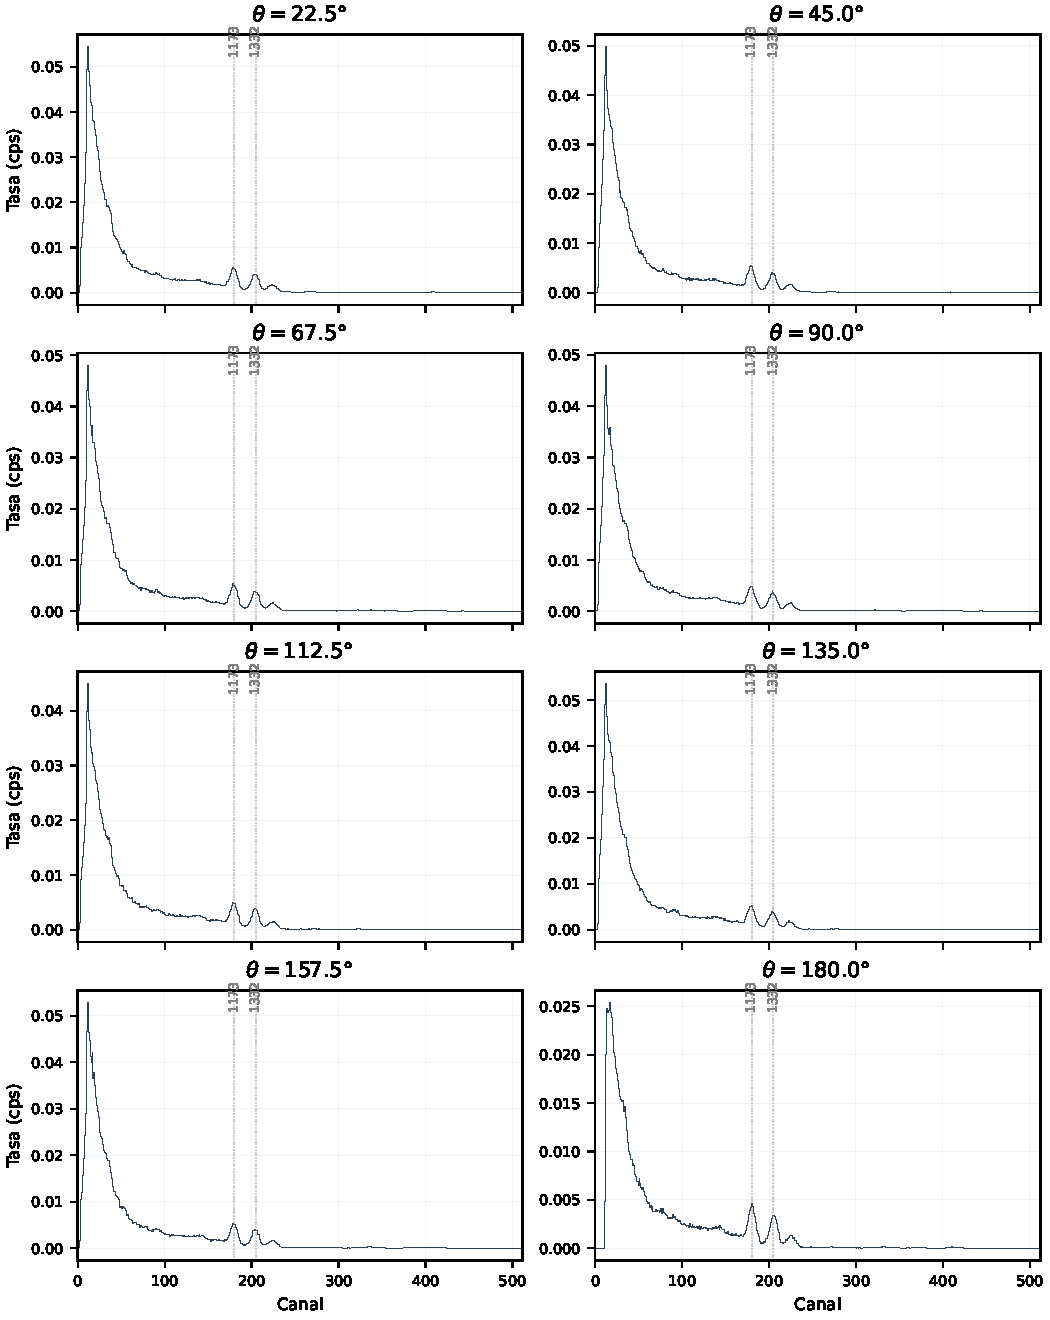
\includegraphics[width=\textwidth, height=0.82\textheight, keepaspectratio]{espectros_individuales.pdf}
  \caption{Espectros de coincidencia $^{60}$Co normalizados por tiempo vivo
           para cada \'angulo (detector m\'ovil, MCAch1).}
  \label{fig:individuales}
\end{figure}

\section{Metodolog\'ia}

Se siguieron los tres pasos descritos en \texttt{Coincidencias/instrucciones.md}:

\begin{enumerate}
  \item \textbf{Cuentas netas.} Para cada \'angulo, se ajustan los picos de
        1173~keV y 1332~keV del espectro en coincidencia (MCAch1) mediante el
        programa Fortran \texttt{gaussian\_background.f}, que realiza una
        sustracci\'on de fondo lineal y un ajuste cuadr\'atico a los datos
        logar\'itmicos. Se obtienen el \'area integrada $A_{pk}$, la amplitud
        $A$ y el ancho $\sigma$.

  \item \textbf{Tasa neta.} El \'area se divide por el tiempo vivo $t_{\text{vivo}}$
        de la medici\'on para obtener la tasa neta:
        \[
        n(\theta) = \frac{A_{pk}}{t_{\text{vivo}}}.
        \]
        El error se propaga desde la matriz de covarianza del ajuste:
        \[
        \Delta n = \frac{\Delta A_{pk}}{t_{\text{vivo}}},
        \qquad
        \Delta A_{pk} = \sqrt{2\pi}\,
        \sqrt{(\sigma\,\Delta A)^2 + (A\,\Delta\sigma)^2}.
        \]

  \item \textbf{Anisotrop\'ia.} Se define la funci\'on de anisotrop\'ia
        normalizando al \'angulo de $90^\circ$:
        \[
        \varepsilon(\theta) = \frac{n(\theta) - n(90^\circ)}{n(90^\circ)},
        \qquad
        \Delta\varepsilon_{\text{areas}} = \sqrt{
        \left(\frac{1}{n_{90}}\right)^{\!2} \! [\Delta n(\theta)]^2 +
        \left(\frac{n(\theta)}{n_{90}^2}\right)^{\!2} \! [\Delta n_{90}]^2 }.
        \]
        La incertidumbre angular por extensi\'on finita de los detectores se
        propaga como $\Delta\varepsilon_{\text{\'ang}} = |d\varepsilon/d\theta|\,
        \Delta\theta$, con $\Delta\theta \approx r_{\text{det}}/R$, resultando
        en el error total:
        \[
        \Delta\varepsilon_{\text{tot}} = \sqrt{
        \Delta\varepsilon_{\text{areas}}^2 +
        \Delta\varepsilon_{\text{\'ang}}^2 }.
        \]
\end{enumerate}

\section{Espectros de coincidencia}

La Figura~\ref{fig:espectros} muestra los espectros de coincidencia del
$^{60}$Co para los ocho \'angulos medidos, con ambos picos identificados.

\begin{figure}[ht]
  \centering
  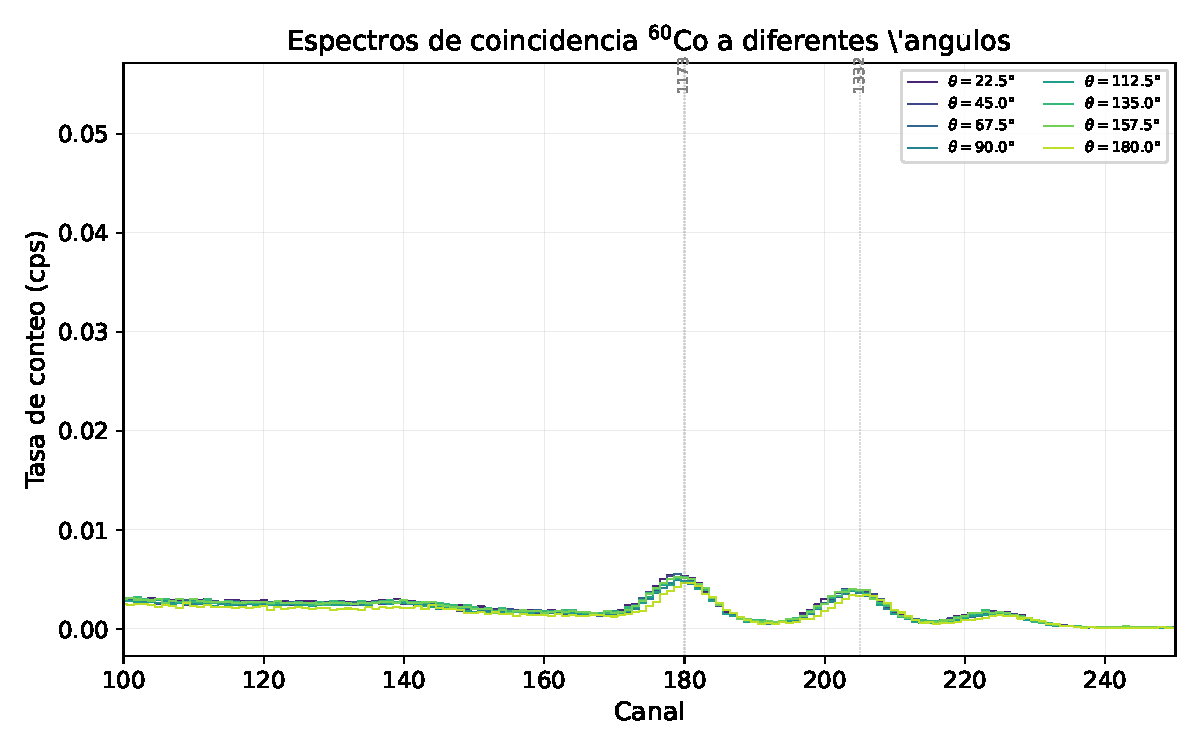
\includegraphics[width=\textwidth]{espectros_superpuestos.pdf}
  \caption{Espectros de coincidencia $^{60}$Co normalizados por tiempo vivo,
           detector m\'ovil (MCAch1). Las l\'ineas punteadas marcan las
           posiciones de los picos de 1173~keV y 1332~keV.}
  \label{fig:espectros}
\end{figure}

\newpage
\section{Resultados detallados}

\subsection{Pico de 1173 keV}

La Tabla~\ref{tab:parametros_1173} muestra los par\'ametros del ajuste
gaussiano y las cantidades derivadas para el pico de 1173~keV.

\begin{table}[ht]
  \centering
  \caption{Par\'ametros del ajuste — pico 1173~keV.}
  \label{tab:parametros_1173}
  \small
  \begin{tabular}{c|c|c|c|c}
    \hline
    $\theta$ & $A$ & $\sigma$ (can.) & \'{A}rea & $n$ (cps) \\
    \hline
    22.5$^\circ$  & $1123 \pm 14$ & $3.68 \pm 0.03$ & $10344 \pm 165$ & $0.0402 \pm 0.0006$ \\
    45$^\circ$    & $744 \pm 12$  & $3.65 \pm 0.04$ & $6817 \pm 133$  & $0.0394 \pm 0.0008$ \\
    67.5$^\circ$  & $728 \pm 11$  & $3.76 \pm 0.04$ & $6858 \pm 134$  & $0.0399 \pm 0.0008$ \\
    90$^\circ$    & $979 \pm 13$  & $3.79 \pm 0.04$ & $9311 \pm 155$  & $0.0359 \pm 0.0006$ \\
    112.5$^\circ$ & $664 \pm 11$  & $3.66 \pm 0.05$ & $6085 \pm 127$  & $0.0353 \pm 0.0007$ \\
    135$^\circ$   & $706 \pm 11$  & $3.81 \pm 0.05$ & $6743 \pm 135$  & $0.0391 \pm 0.0008$ \\
    157.5$^\circ$ & $1087 \pm 14$ & $3.63 \pm 0.03$ & $9878 \pm 161$  & $0.0382 \pm 0.0006$ \\
    180$^\circ$   & $622 \pm 11$  & $3.65 \pm 0.04$ & $5700 \pm 117$  & $0.0333 \pm 0.0007$ \\
    \hline
  \end{tabular}
\end{table}

\subsection{Pico de 1332 keV}

La Tabla~\ref{tab:parametros_1332} muestra los par\'ametros para el pico de
1332~keV.

\begin{table}[ht]
  \centering
  \caption{Par\'ametros del ajuste — pico 1332~keV.}
  \label{tab:parametros_1332}
  \small
  \begin{tabular}{c|c|c|c|c}
    \hline
    $\theta$ & $A$ & $\sigma$ (can.) & \'{A}rea & $n$ (cps) \\
    \hline
    22.5$^\circ$  & $822 \pm 13$ & $3.84 \pm 0.05$ & $7903 \pm 162$ & $0.0307 \pm 0.0006$ \\
    45$^\circ$    & $562 \pm 10$ & $3.64 \pm 0.05$ & $5130 \pm 119$ & $0.0297 \pm 0.0007$ \\
    67.5$^\circ$  & $551 \pm 10$ & $3.86 \pm 0.06$ & $5328 \pm 125$ & $0.0310 \pm 0.0007$ \\
    90$^\circ$    & $777 \pm 12$ & $3.70 \pm 0.05$ & $7197 \pm 145$ & $0.0277 \pm 0.0006$ \\
    112.5$^\circ$ & $536 \pm 10$ & $3.70 \pm 0.06$ & $4976 \pm 120$ & $0.0289 \pm 0.0007$ \\
    135$^\circ$   & $533 \pm 10$ & $3.69 \pm 0.05$ & $4934 \pm 119$ & $0.0286 \pm 0.0007$ \\
    157.5$^\circ$ & $838 \pm 13$ & $3.69 \pm 0.05$ & $7751 \pm 153$ & $0.0299 \pm 0.0006$ \\
    180$^\circ$   & $492 \pm 9$  & $3.82 \pm 0.06$ & $4709 \pm 113$ & $0.0275 \pm 0.0007$ \\
    \hline
  \end{tabular}
\end{table}

\newpage
\subsection{Resumen de tasas netas}

La Tabla~\ref{tab:tasas} compara las tasas netas $n(\theta)$ de ambos picos.

\begin{table}[ht]
  \centering
  \caption{Tasas netas $n(\theta)$ (cps) para ambos picos.}
  \label{tab:tasas}
  \small
  \begin{tabular}{c|c|c|c}
    \hline
    $\theta$ & $n_{1173}$ (cps) & $n_{1332}$ (cps) & $t_{\text{vivo}}$ (s) \\
    \hline
    22.5$^\circ$  & $0.0402 \pm 0.0006$ & $0.0307 \pm 0.0006$ & 257547 \\
    45$^\circ$    & $0.0394 \pm 0.0008$ & $0.0297 \pm 0.0007$ & 172902 \\
    67.5$^\circ$  & $0.0399 \pm 0.0008$ & $0.0310 \pm 0.0007$ & 171995 \\
    90$^\circ$    & $0.0359 \pm 0.0006$ & $0.0277 \pm 0.0006$ & 259698 \\
    112.5$^\circ$ & $0.0353 \pm 0.0007$ & $0.0289 \pm 0.0007$ & 172204 \\
    135$^\circ$   & $0.0391 \pm 0.0008$ & $0.0286 \pm 0.0007$ & 172658 \\
    157.5$^\circ$ & $0.0382 \pm 0.0006$ & $0.0299 \pm 0.0006$ & 258852 \\
    180$^\circ$   & $0.0333 \pm 0.0007$ & $0.0275 \pm 0.0007$ & 170965 \\
    \hline
  \end{tabular}
\end{table}

\subsection{Anisotrop\'ia}

La Tabla~\ref{tab:anisotropia} muestra la anisotrop\'ia
$\varepsilon(\theta) = [n(\theta)-n(90^\circ)]/n(90^\circ)$
para ambos picos y la Figura~\ref{fig:anisotropia} su representaci\'on gr\'afica.

\begin{table}[ht]
  \centering
  \caption{Anisotrop\'ia $\varepsilon(\theta)$ para ambos picos.
           El error incluye la contribuci\'on estad\'istica y la
           incertidumbre angular por extensi\'on finita de los detectores.}
  \label{tab:anisotropia}
  \small
  \begin{tabular}{c|c|c}
    \hline
    $\theta$ & $\varepsilon_{1173}$ & $\varepsilon_{1332}$ \\
    \hline
     22.5$^\circ$  & $0.1203 \pm 0.0282$ & $0.1072 \pm 0.0338$ \\
     45$^\circ$    & $0.0996 \pm 0.0313$ & $0.0706 \pm 0.0356$ \\
     67.5$^\circ$  & $0.1122 \pm 0.0296$ & $0.1178 \pm 0.0354$ \\
     90$^\circ$    & $0.0000 \pm 0.0235$ & $0.0000 \pm 0.0284$ \\
     112.5$^\circ$ & $-0.0144 \pm 0.0275$ & $0.0426 \pm 0.0337$ \\
     135$^\circ$   & $0.0892 \pm 0.0315$ & $0.0311 \pm 0.0351$ \\
     157.5$^\circ$ & $0.0644 \pm 0.0273$ & $0.0804 \pm 0.0324$ \\
     180$^\circ$   & $-0.0701 \pm 0.0245$ & $-0.0061 \pm 0.0312$ \\
    \hline
  \end{tabular}
\end{table}

\begin{figure}[ht]
  \centering
  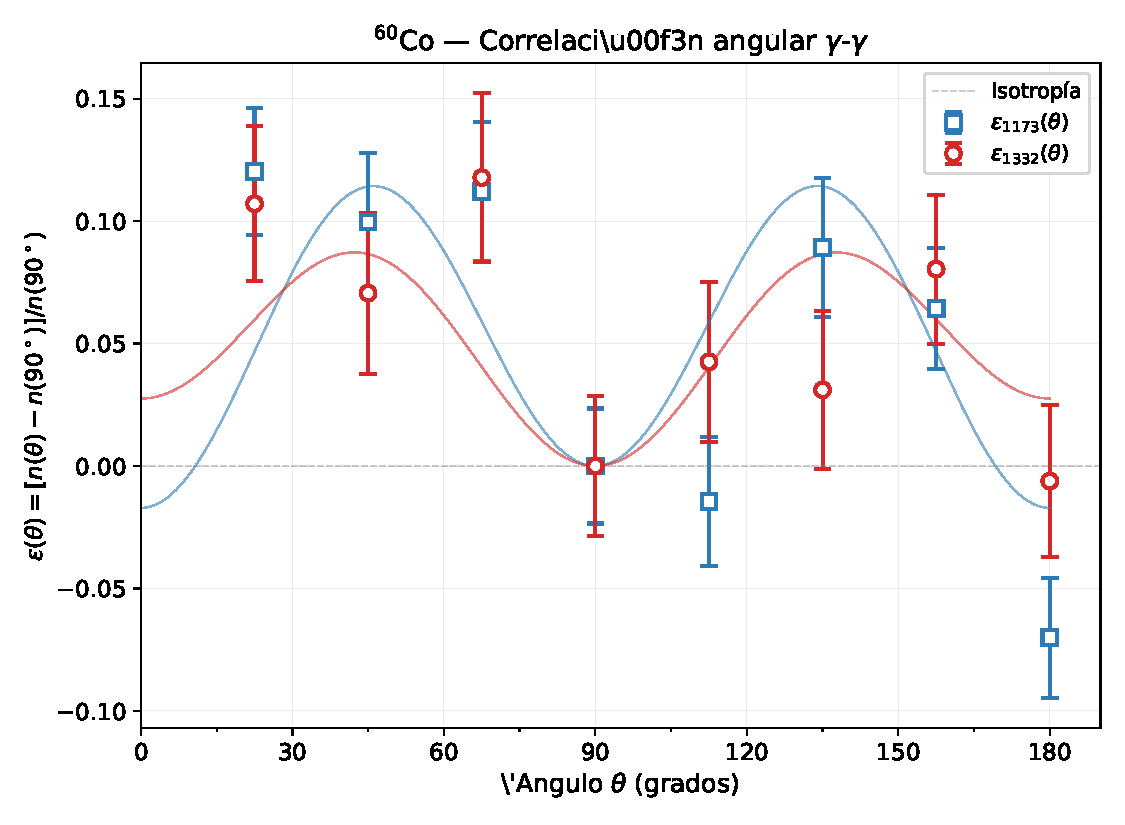
\includegraphics[width=0.8\textwidth]{anisotropia.pdf}
  \caption{Anisotrop\'ia $\varepsilon(\theta)$ para los picos de 1173~keV y
           1332~keV. Las barras de error representan $1\sigma$.}
  \label{fig:anisotropia}
\end{figure}

\subsection{Comparaci\'on detector fijo vs.\ m\'ovil}

La Figura~\ref{fig:comparacion} muestra los espectros de coincidencia de ambos
detectores para cada \'angulo. El detector fijo (MCAch0) permanece a $90^\circ$
mientras que el m\'ovil (MCAch1) se desplaza al \'angulo indicado. Ambos
espectros est\'an normalizados por tiempo vivo.

\begin{figure}[ht]
  \centering
  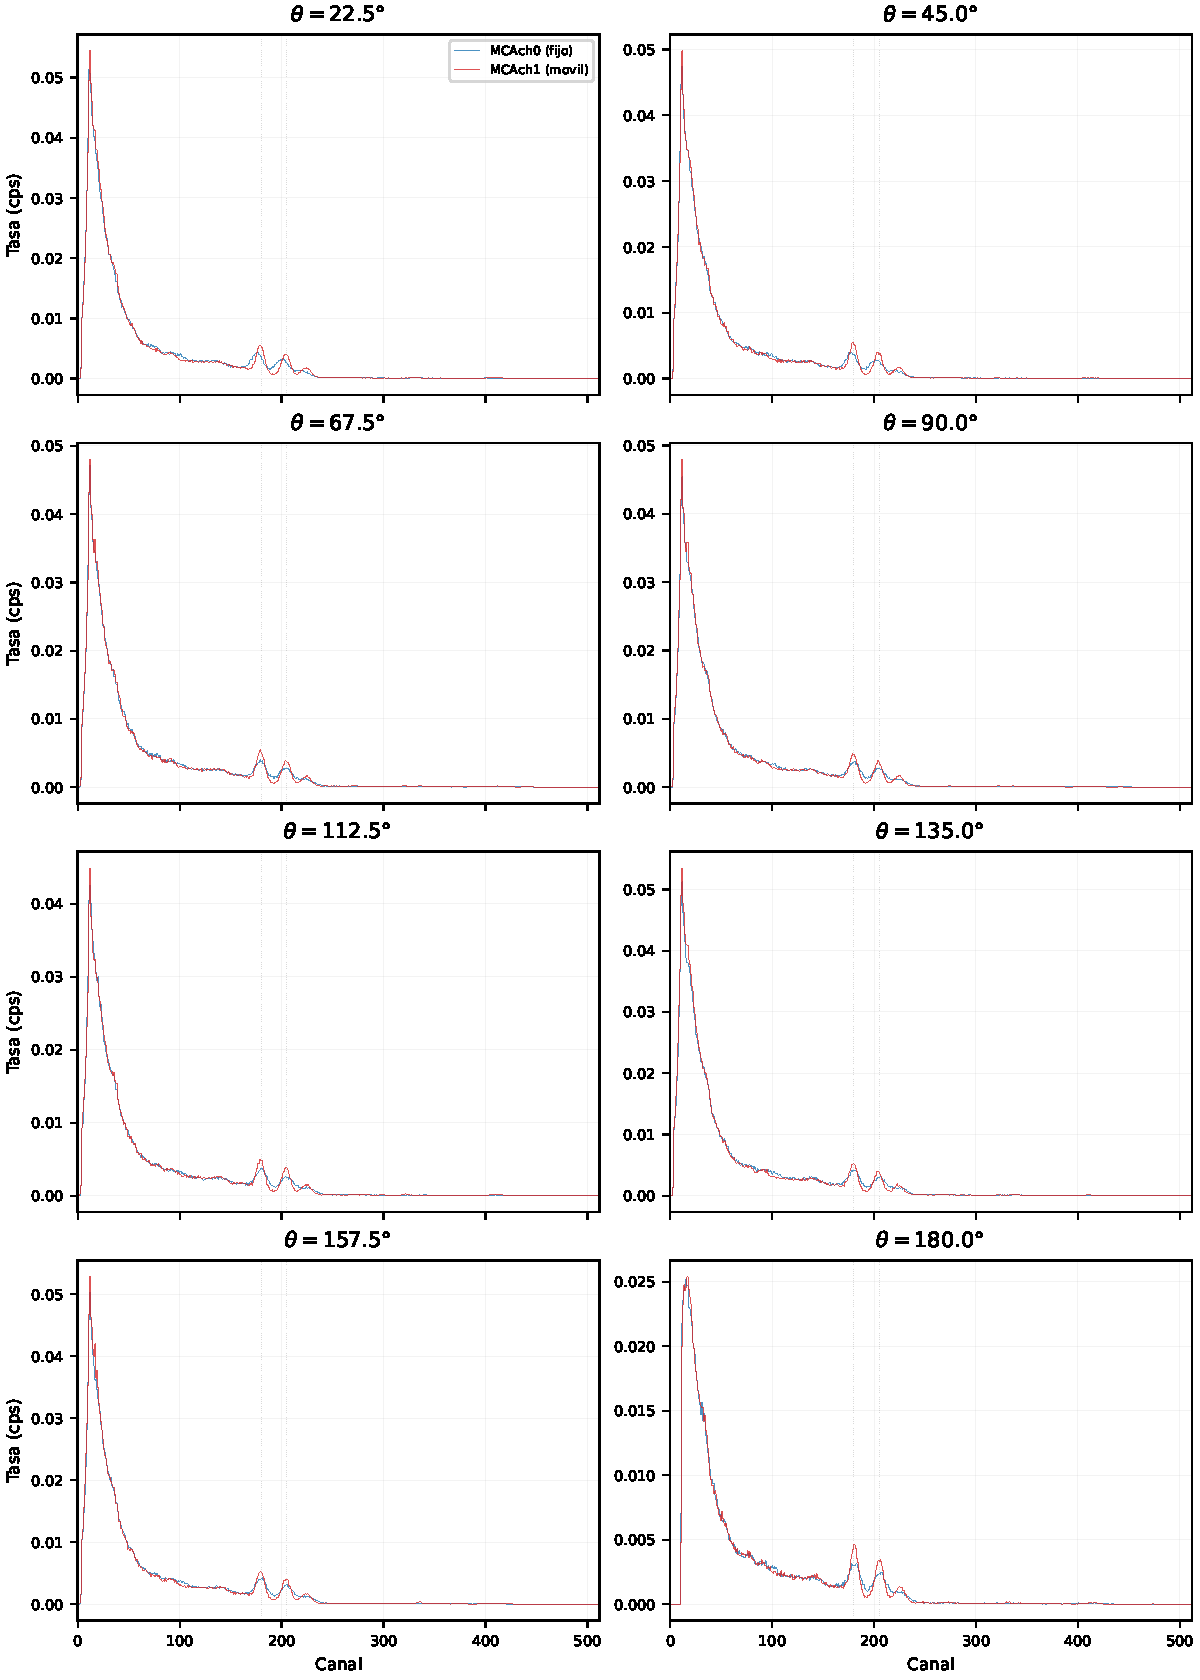
\includegraphics[width=\textwidth]{comparacion_fijo_movil.pdf}
  \caption{Espectros de coincidencia del detector fijo (MCAch0, $90^\circ$)
           y el m\'ovil (MCAch1) normalizados por tiempo vivo.
           Las l\'ineas punteadas marcan las posiciones de 1173~keV y
           1332~keV.}
  \label{fig:comparacion}
\end{figure}

\newpage
\section{Discusi\'on}

Los valores de anisotrop\'ia normalizados a $90^\circ$ muestran una
variaci\'on relativa de hasta $\sim$12\,\% respecto al \'angulo de referencia.
Para el pico de 1332~keV, $\varepsilon$ var\'ia entre $-0.01$ y $+0.12$, con
un m\'aximo en torno a $67.5^\circ$ y valores m\'inimos hacia $90^\circ$ y
$180^\circ$. Para el pico de 1173~keV, la variaci\'on es similar ($-0.07$ a
$+0.12$), con un perfil comparable pero con una ca\'ida m\'as marcada a
$180^\circ$ ($\varepsilon = -0.07$).

Ambos picos pertenecen a la misma cascada $\gamma$--$\gamma$
$4^+ \xrightarrow{1173\,\text{keV}} 2^+
\xrightarrow{1332\,\text{keV}} 0^+$, por lo que deber\'ian presentar la misma
correlaci\'on angular. Las diferencias observadas pueden deberse a:

\begin{itemize}
  \item Mayor interferencia del fondo Compton debajo del pico de 1173~keV
        (el pico de 1332~keV est\'a m\'as aislado).
  \item Contribuci\'on de la cola del pico de 1173~keV al fondo del 1332~keV,
        y viceversa, que el ajuste con fondo lineal no separa completamente.
  \item Estad\'istica limitada en algunos \'angulos (errores de $\sim$2--3\,\%).
\end{itemize}

Los errores t\'ipicos del \'area integrada son del orden del 2\,\% para ambos
picos, propag\'andose a errores en $\varepsilon$ de $\sim$3\,\%. A estos
se suma la incertidumbre angular por extensi\'on finita de los detectores
($\Delta\varepsilon_{\text{\'ang}}$), comparable o mayor que la estad\'istica
en los \'angulos donde $|d\varepsilon/d\theta|$ es grande.

\subsection{Correcci\'on por \'angulo s\'olido finito}

Los detectores tienen tama\~no finito, por lo que la correlaci\'on angular
observada se aten\'ua respecto a la de detectores puntuales. La correcci\'on
se realiza mediante los factores $Q_k$, que para detectores coaxiales
cil\'indricos se aproximan como:

\[
Q_k \approx \frac{\int_{0}^{\beta_0} P_k(\cos\beta) \sin\beta \, d\beta}
{\int_{0}^{\beta_0} \sin\beta \, d\beta},
\qquad
\beta_0 = \arctan\left(\frac{r}{R}\right),
\]

siendo $R = 0.5$~m la distancia fuente-detector y $d = 81.8$~mm el di\'ametro
del cristal de NaI. Con $\beta_0 = 4.68^\circ$, las integrales anal\'iticas dan:

\[
Q_2 = \frac{\cos\beta_0(1+\cos\beta_0)}{2} = 0.9950,
\qquad
Q_4 = \frac{\cos\beta_0(1+\cos\beta_0)(7\cos^2\beta_0 - 3)}{8} = 0.9834.
\]

Como ambos detectores son id\'enticos, el factor de correcci\'on total es
$Q_k^2$, resultando en $Q_2^2 = 0.9900$ y $Q_4^2 = 0.9672$. La correcci\'on
es peque\~na (1\,\% y 3\,\%) y est\'a dentro de los errores estad\'isticos.

La incertidumbre angular por extensi\'on finita de los detectores se propaga
como $\Delta\varepsilon_{\text{\'ang}} = |d\varepsilon/d\theta|\,\Delta\theta$,
con $\Delta\theta \approx r_{\text{det}}/R = 0.0818$~rad. Tomando la expresi\'on
te\'orica de la correlaci\'on angular del $^{60}$Co se obtiene:

\[
\frac{d\varepsilon}{d\theta} = \frac{1}{4}\cos\theta\,\sin\theta
+ \frac{1}{6}\cos^3\theta\,\sin\theta,
\qquad
\Delta\varepsilon_{\text{\'ang}} = \left|\,
\frac{1}{4}\cos\theta\,\sin\theta
+ \frac{1}{6}\cos^3\theta\,\sin\theta\,\right|\,
\frac{r_{\text{det}}}{R}.
\]

Los datos de anisotrop\'ia se ajustaron a la funci\'on:

\[
\varepsilon(\theta) = \frac{1 + \alpha_2 P_2(\cos\theta) + \alpha_4 P_4(\cos\theta)}
{1 + \alpha_2 P_2(0) + \alpha_4 P_4(0)} - 1,
\qquad
P_2(x) = \frac{3x^2 - 1}{2},\;
P_4(x) = \frac{35x^4 - 30x^2 + 3}{8}.
\]

La Tabla~\ref{tab:coeficientes} muestra los coeficientes observados
$\alpha_k = Q_k^2 a_k$ y los corregidos $a_k = \alpha_k / Q_k^2$.
Las curvas del ajuste se superponen en la Figura~\ref{fig:anisotropia}.

\begin{table}[ht]
  \centering
  \caption{Coeficientes de Legendre observados y corregidos por \'angulo s\'olido.}
  \label{tab:coeficientes}
  \small
  \begin{tabular}{c|c|c|c|c}
    \hline
    Pico & $\alpha_2$ & $\alpha_4$ & $a_2^{\text{corr}}$ & $a_4^{\text{corr}}$ \\
    \hline
    1173~keV & $0.0334 \pm 0.0091$ & $-0.1059 \pm 0.0174$ &
              $0.0337 \pm 0.0092$ & $-0.1095 \pm 0.0180$ \\
    1332~keV & $0.0440 \pm 0.0114$ & $-0.0635 \pm 0.0214$ &
              $0.0444 \pm 0.0115$ & $-0.0657 \pm 0.0221$ \\
    \hline
  \end{tabular}
\end{table}

\end{document}
